\section{Bluetooth Low Energy}
\subsection{Présentation}
\begin{frame}
	\begin{minipage}[t]{0.45\linewidth}
	\uncover<2->{
		\begin{figure}
			\includegraphics[height=3.25cm]{img/bt_logo_smart_and_ready.jpg}
			\caption{Logos Bluetooth Low Energy}
		\end{figure}
	}
	\end{minipage}
	\begin{minipage}[t]{0.52\linewidth}
		\uncover<1->{
		\begin{block}{Bluetooth Smart}
			\begin{itemize}
				\item 2006 : Wibree ( Nokia )
				\item 2010 : Bluetooth 4.0
			\end{itemize}
		\end{block}
		}
		\uncover<3->{
		\begin{block}{Caractéristiques}
			\begin{itemize}
				\item 2.4 GHz
				\item 40 cannaux
				\item 1 Mbit/s
				\item Conso entre 0.01W et 0.5W
			\end{itemize}
		\end{block}
		}
	\end{minipage}
\end{frame}

\subsection{Architecture logique}
\begin{frame}


\begin{minipage}[t]{0.47\linewidth}
	\begin{figure}
		\includegraphics[height=6cm]{img/arch_core.png}
		\caption{Core BR/EDR}
	\end{figure}
\end{minipage}
\begin{minipage}[t]{0.45\linewidth}
	\begin{figure}
		\includegraphics[height=6cm]{img/arch_core_ble.png}
		\caption{Core BLE}
	\end{figure}
\end{minipage}
% ici schema diff BT/BLE de bt.org
\end{frame}
\begin{frame}

\begin{minipage}[t]{0.47\linewidth}
	\begin{figure}
		\includegraphics[height=6cm]{img/arch_core_ble.png}
		\caption{Core BLE}
	\end{figure}
\end{minipage}
\begin{minipage}[t]{0.45\linewidth}
	\begin{block}{Link Layer}
		\begin{itemize}
			\item Advertising
			\item Scanning
			\item Connected
		\end{itemize}
	\end{block}
	\begin{block}{Sécurité}
		\begin{itemize}
			\item Clé côté Host
			\item AES 128
			\item Adresses :
			\begin{itemize}
				\item Publique
				\item Aléatoire
			\end{itemize}
		\end{itemize}
	\end{block}
\end{minipage}
% ici schema diff BT/BLE de bt.org
\end{frame}

\begin{frame}
	\begin{minipage}[t]{0.60\linewidth}
		\uncover<1->{
			\begin{figure}
				\includegraphics[height=5cm]{img/arch_log_all_ble.png}
				\caption{ATTributes / Generic ATTributes}
			\end{figure}
		}
	\end{minipage}
	\begin{minipage}[t]{0.38\linewidth}
		\uncover<2->{
		\begin{block}{ATT}
			\begin{itemize}
				\item Protocole
				\item Transport d'attributs
			\end{itemize}
		\end{block}
		}
		\uncover<3->{
		\begin{block}{GATT}
			Profil BLE
			\begin{itemize}
				\item Client
				\item Serveur
			\end{itemize}
		\end{block}
		}
	\end{minipage}
\end{frame}


\subsection{Attributs}
\begin{frame}
\begin{columns}[t]
\begin{column}{0.45\linewidth}
\begin{center} \huge GATT \end{center}
	\uncover<2->{
	\begin{block}{Attribut}
		\begin{itemize}
			\item Type : UUID
			\item Permissions : \begin{itemize}
						\item R/W
						\item Encryption
						\item Autorisation
					\end{itemize}
			\item Valeur
			\item Handle : Adresse
		\end{itemize}
	\end{block}
}
\end{column}
\begin{column}[t]{0.45\linewidth}
	\uncover<3->{
	\begin{block}{Services}
		\uncover<4->{
		Regroupe des :
		\begin{columns}[T]
		\begin{column}{0.90\textwidth}
		\begin{block}{Caractéristiques}
			\uncover<5->{
			\begin{itemize}
				\item Déclaration
				\item Valeur
				\item<6-> Et parfois :
			\end{itemize}
			\begin{columns}[T]
			\begin{column}{0.90\textwidth}
				\uncover<7->{
					\vspace{-0.5cm}
			\begin{block}{Descripteurs}
			Métadonnées sur la caractéristique
		}
			\end{block}
		}
			\end{column}
			\end{columns}
		\end{block}
		\end{column}
		\end{columns}
	}
	\end{block}
}
\end{column}
\end{columns}
\end{frame}

\begin{frame}
	\begin{figure}
		\includegraphics[height=5cm]{img/gatt.png}
		\caption{Exemple de service GATT}
	\end{figure}
{\tiny "Getting started with bluetooth low energy", R.Davidson, Akiba, Carles Cufí, Kevin Townsend, O'Reilly}
\end{frame}
